\section{Quantum Double Model III}
\subsection{Ground State of QD Model}
We recall the QD model with group $G$, with local Hilbert spaces on edges of a lattice of dimension $\abs{G}$, and Hamiltonian given by:
\begin{equation}
    H = -\sum_s A(s) - \sum_p B(p)
\end{equation}
with the star term:
\begin{equation}
    A(s) = \frac{1}{\abs{G}}\sum_g A_g(s)
\end{equation}
and $A_g(s)$ corresponding to a left-multiplication of $g$ on each of the inward pointing legs, and $B(p)$ the plaquette term the projector onto the subspace with $h_1h_2h_3h_4 = 1$ (product of group elements around the plaquette) - whether the flux through the plaquette is vanishing/1 (we can also consider $B_h(p)$ which checks that the flux is equal to a group element $h$). We showed last time that the $\set{A(s), B(p)}$ are all projectors and mutually commute. It is thus easy to find the ground states:
\begin{equation}
    A(s)\ket{\Omega} = B(p)\ket{\Omega} = \ket{\Omega}
\end{equation}
i.e. they should be the $+1$ eigenstates of all of the commuting projectors in order to be the lowest energy eigenstate. Now, we can ask; how many ground states are there in the infinite plane geometry?

\begin{equation}
    B(p)\ket{\Omega} = \ket{\Omega} \implies \ket{\Omega} \text{ is a sum of states $\ket{\set{g_j}}$ with vanishing ($=1$) flux}
\end{equation}

At the end of last lecture we wrote down a couple examples of such vanishing flux states. The statement we make above is that we can form any arbitrary linear combination of vanishing flux states, and they will have $B(p)\ket{\Omega} = (+1)\ket{\Omega}$ for all $p$. For now, the coefficients in this linear combinations are arbitrary. This will fix the coefficients (very similar to what we did in the toric code case).

We now want to impose the constraint $A(s)\ket{\Omega} = \ket{\Omega}$. We now make a claim that this is equivalent to saying that $A_g(s)\ket{\Omega} = \ket{\Omega}$ for all $g$. The $A_g(s) = +1 \implies A(s) = +1$ direction is clear. The other direction is not quite as obvious, but it is a straightforwards to show, and you will do it on the homework. 

Because $A_g(s)$ imposes a gauge transformation, it being $+1$ implies that the amplitude of the pre-gauge transformed and post-transformed states must be the same in the states. More concretely, $A_g(s)\ket{\Omega} = \ket{\Omega}$ implies that:
\begin{equation}
    \bra{\set{g_j}}A_g(s)\ket{\Omega} = \braket{\set{g_j}}{\Omega}
\end{equation}
acting on the left with $A_g(s)$:
\begin{equation}
    \bra{\set{g_j'}}A_g(s)\ket{\Omega} = \braket{\set{g_j}}{\Omega}
\end{equation}
and hence any two basis states related by a gauge transformation/$A_g(s)$ must have the same amplitude if we are to have $A(s)\ket{\Omega} = \ket{\Omega}$. Now, the key obervation is that all of the zero flux states are related by a gauge transformation (the gauge transformations are ergodic); if we again look at our examples:
\begin{center}
    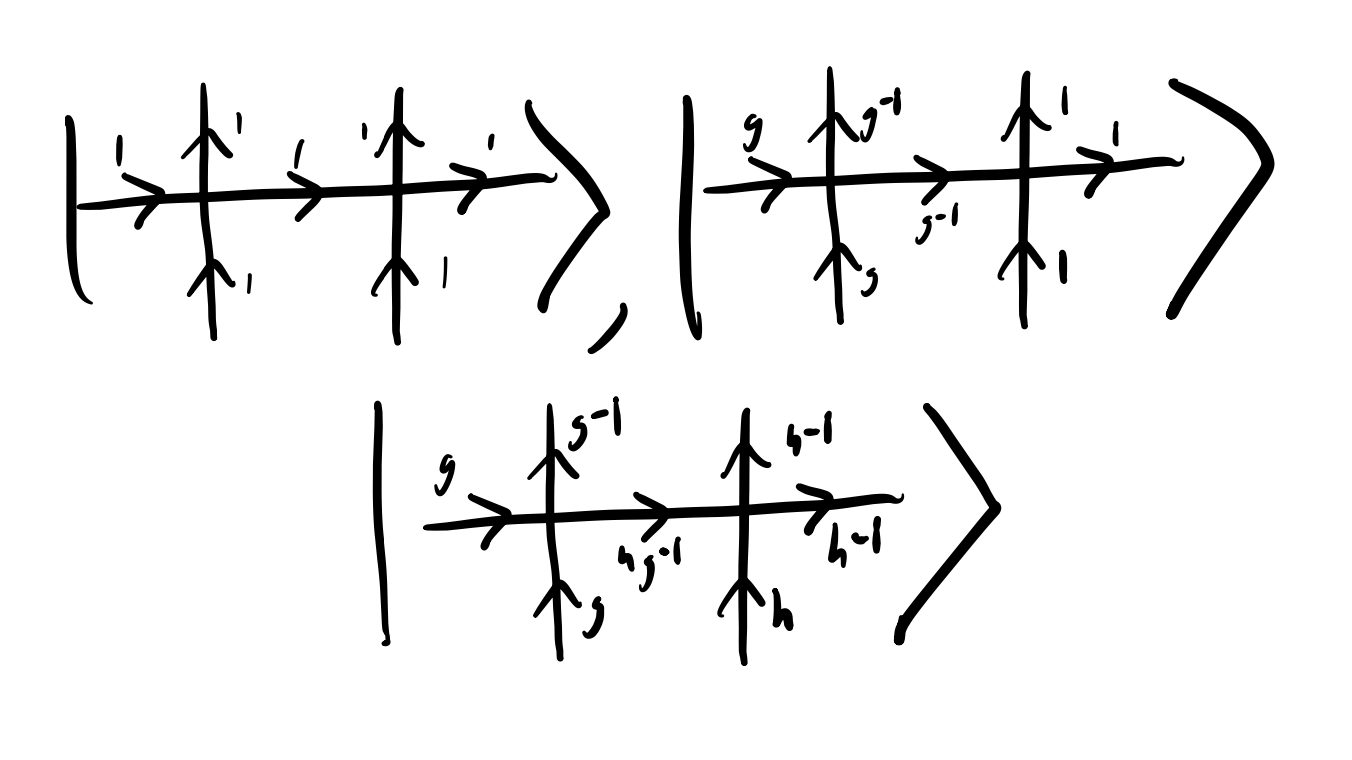
\includegraphics[scale=0.35]{Lectures/Images/lec7-nofluxstates.png}
\end{center}
this becomes clear. The second state is related by a $g$ transformation to the first, and the third state is related to the second by a $h$ transformation. Note that this observation that all zero-flux states are connectable is specific to the infinite plane geometry.

The conclusion of the arguments; $\ket{\Omega}$ is an equal weight superposition of all vanishing flux states\footnote{analogous to the Toric code result where we had an equal weight superposition of all closed loop states}
\begin{equation}
    \ket{\Omega} = \sum_{\set{g_j} \text{ vanishing flux}} \ket{\set{g_j}}
\end{equation}

A notable comment - out of this analysis, we have found that the ground state is unique. Furthermore, the lowest excited states have $A(s) = 0$ or $B(p) = 0$ for some $s, p$. The energy gap (though we do not show it here) is therefore $\Delta = 1$. So, this is another example of a gapped Hamiltonian, and this is the setting where the notion of anyons are well-defined.

\subsection{General Definition of Anyons}
This is one of the most interesting aspects of the quantum double model. In particular, it is a nice toy model for introducing non-abelian anyons. We have associated anyons with excitations of a Hamiltonian, but this is a bit of a misnomer. Let's more precisely define it.

\emph{Definition (Anyons).} An ``anyon excitation'' of a gapped (local) Hamiltonian $H_0$ is any state which is the unique ground state of the of a Hamiltonian of the following form:
\begin{equation}
    H = H_0 + V
\end{equation}
with $V$ a local (Hermitian) operator. We can call this a trapping potential\footnote{We think about the infinite plane here, where we have one anyon somewhere and another anyon at infinity. We could also think about this with a pair of anyons created by two trapping potentials.}.

The physical idea - if $H_0$ has ground state $\ket{\Omega}$, then the ground state of $H$ looks like $\ket{\Omega}$ plus a perturbation/localized defect near $V$. We can trap these excitations locally, but we \emph{cannot} create them locally.

\emph{Definition (Equivalent anyons).}Two anyon excitations $\ket{\psi}, \ket{\psi'}$ (corresponding to potentials $V, V'$) are equivalent/the same (topological) ``type'' if $\ket{\psi} = U\ket{\psi}$ for some local unitary $U$ (supported near $V$).

We can see that this is a reasonable definition by looking at the $e, m$ anyons of the toric code. There, we have different choices of $V$ we can take:
\begin{itemize}
    \item ($V = 0$): $H = -\sum_s A_s - \sum_p B_p$ (``1'' anyon)
    \item ($V = 2A_{s_0}$): $H = -\sum_{s \neq s_0} A_s - \sum_p B_p + A_{s_0}$ (``$e$'' anyon)
    \item ($V = 2B_{p_0}$): $H = -\sum_s A_s - \sum_{p\neq p_0} B_p + B_{p_0}$ (``$m$'' anyon)
    \item ($V = 2A_{s_0} + 2B_{p_0}$): $H = -\sum_{s \neq s_0} A_s - \sum_{p \neq p_0} B_p + A_{s_0} + B_{p_0}$ (``$\e$'' anyon)
\end{itemize}
Every other kind of anyon we could create are equivalent up to a local unitary $U$. For example two ``$e$''s are equivalent to the trivial anyon via a local string operator connecting them.

\subsection{Flux anyons of Quantum Double Model}
The QD model will turn out to have analogs of all of the toric code excitations. We will start by thinking about the flux excitations (generalization of toric code ``$m$'').

First, we can ask how many types of flux excitations there are. Claim: For a general group $G$, there is one type of flux exicitation for every non-trivial conjugacy class $C \subset G$ (the equivalence classes of a group under the relation of conjugation). For each one of these classes, we can construct a distinct flux excitation.

We will proceed by defining a different trapping potential $V$ for each conjugacy class and showing that the $H_0 + V$ has a unique ground state, which cannot be related to each other via local operation.

We consider the modified quantum double Hamiltonian:
\begin{equation}\label{eq:modifiedQD}
    H = -\sum_s A(s) - \sum_{p \neq p_0}B(p) - B_C(p_0)
\end{equation}
So the trapping potential is:
\begin{equation}
    V(p_0) = B(p_0)- B_C(p_0)
\end{equation}
with $B_C(p_0)$ defined for each conjugacy class $C \subseteq G$:

\begin{center}
    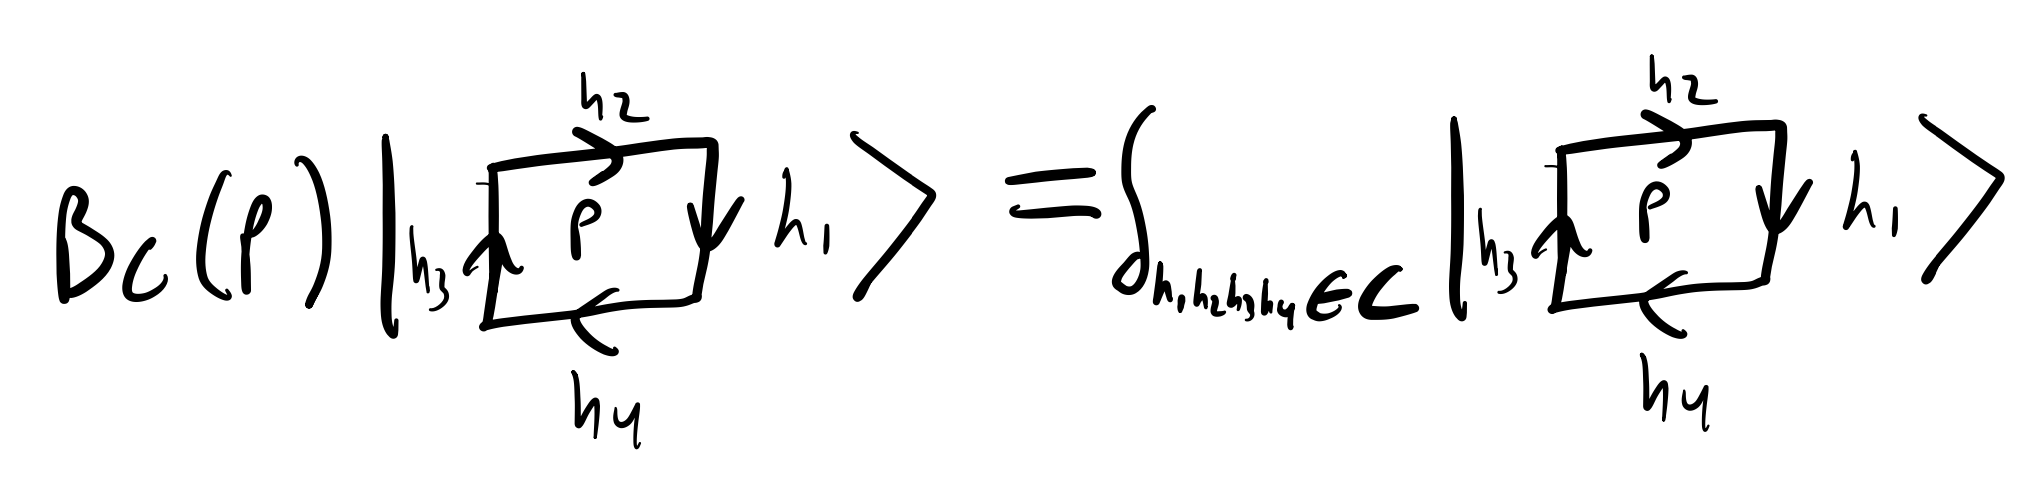
\includegraphics[scale=0.35]{Lectures/Images/lec8-Bcp.png}
\end{center}

In other words, $B_C(p_0)$ measures the flux through $p_0$ and checks that the flux lives in the conjugacy class $C$. Note that $B_C(p_0)$ also commutes with $A(s)$ (how to see this? $A(s)$ preserves and/or preserves the flux, and thus commutes with $B_C(p_0)$ which only cares about the conjugacy class of the flux).

So, we can think about the ground state of the Hamiltonian of Eq. \eqref{eq:modifiedQD} as we did for the quantum double model. In particular the analysis of the plaquette operators goes through in the same way, save for the fact that we now require that our states in our superposition all have nonzero flux through $p_0$. Then the $A(s)$ constraints tell us that the states in this superposition have equal weight. We thus again have a unique ground state:
\begin{equation}
    \ket{C} = \sum_{\set{g_j} \text{ flux $C$ through $p_0$, 1 elsewhere}} \ket{\set{g_j}}
\end{equation}

We could ask why didn't we just look for an excited state in the original Hamiltonian. The idea is that all conjugacy class eigenstates have the same excited state energy - there is degeneracy in the excited states. But via the local trapping potential definition we split this degeneracy and can identify the distinct anyon excitations.

We need to now argue that different choices of $C$ give rise to distinct excitations, in the sense that they cannot be connected via a local unitary:
\begin{equation}
    \ket{C'} \neq U\ket{C} \quad (\text{if $C' \neq C$})
\end{equation}
To see this, we define the operator $B_C(\gamma)$, which looks at the conjugacy class of a flux around a large loop:

\begin{center}
    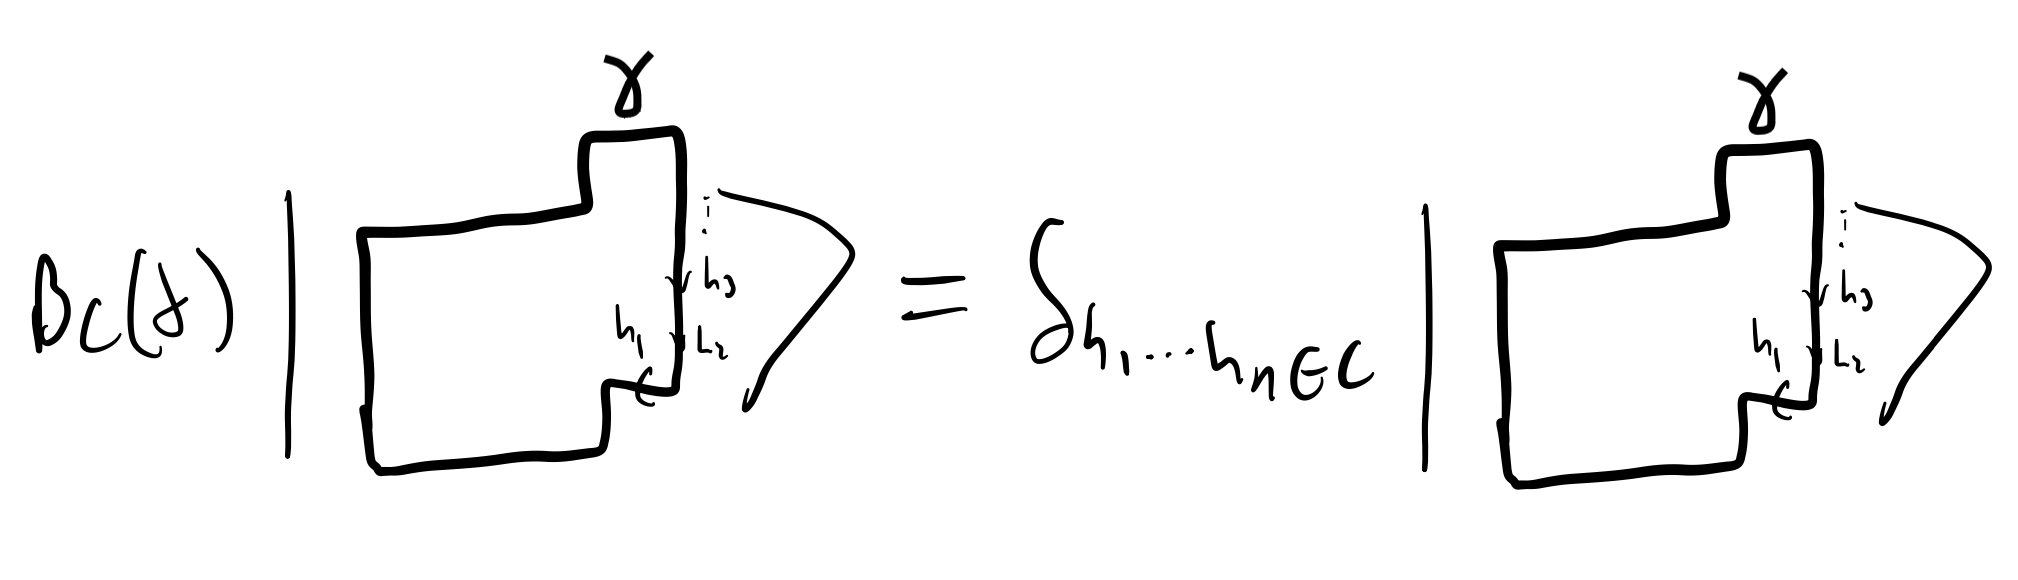
\includegraphics[scale=0.35]{Lectures/Images/lec8-Bcgamma.png}
\end{center}

Then, it follows that:
\begin{equation}
    B_C(\gamma)\ket{C} = \ket{C}
\end{equation}
Which follows from a similar kind of Stokes' theorem that we saw in the toric code case. It can measure the flux inside of the large curve:

\begin{center}
    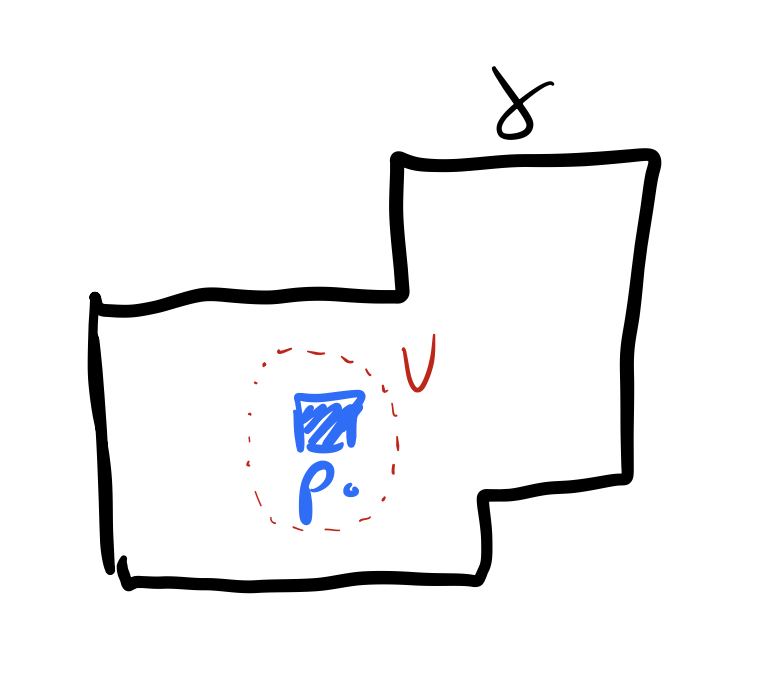
\includegraphics[scale=0.35]{Lectures/Images/lec8-fluxmeasure.png}
\end{center}

But if we have a different conjugacy class:
\begin{equation}
    B_C(\gamma)\ket{C'} = 0
\end{equation}
because it measures the flux inside and sees that it is not equal to $C$. This is sufficient to show that $\ket{C}, \ket{C'}$ cannot be locally connected by a local $U$:
\begin{equation}
    \ket{C'} \neq U\ket{C}.
\end{equation}
Because $\gamma$ can be arbitrarily large, and thus have no overlap with a local $U$ (and hence commute); if the above were true, then:
\begin{equation}
    B_C(\gamma)\ket{C'} = B_C(\gamma)U\ket{C} = UB_C(\gamma)\ket{C} = U\ket{C} \neq 0
\end{equation}
contradiction!

Next time - we will think about trapping $n$ fluxes (rather than trapping a single flux). And then we will see that this has multiple degenerate ground states, which will be the foundation for non-abelian anyons.
